\documentclass[11pt,letterpaper]{article}
\usepackage[margin=1in]{geometry}
\usepackage[T1]{fontenc}
\usepackage[utf8]{inputenc}
\usepackage{amsmath,amssymb,graphicx,booktabs,tabularx,array,caption}
\usepackage{hyperref}
\IfFileExists{microtype.sty}{\usepackage{microtype}}{}
\hypersetup{colorlinks=true,allcolors=black,pdftitle={Optical sampling and alignment uncertainty in a retrospective T4 model assessment}}
\urlstyle{same}
\setlength{\parindent}{0pt}
\setlength{\parskip}{6pt}
\renewcommand{\baselinestretch}{1.06}
\setcounter{secnumdepth}{0}
\widowpenalty=10000
\clubpenalty=10000
\setlength{\emergencystretch}{2em}
\captionsetup{font=small,labelfont=bf}
\begin{document}
\begin{center}
{\Large\bfseries Optical sampling and alignment uncertainty in a retrospective T4 model assessment}
\end{center}
\textbf{Initial research manuscript | 16 November 2026 | Version 1}


This draft reports a completed computational pilot. It contains a retrospective audit of archived stimulus images and a separate simulation with known truth. It does not report new neural recordings or a validated improvement in biological model selection. Authorship, affiliations, funding and other author declarations must be supplied by the investigators before submission.


\section{Abstract}

Comparisons between neural models and recordings depend on how visual stimuli are registered to modeled receptive fields. An earlier reanalysis of a published Drosophila T4 dataset identified model alignments with identical flashed-bar inputs but different motion predictions. We examined whether those input equivalences persisted under alternative spatial sampling and evaluated the consequences of calibration uncertainty in a separate controlled simulation. The archived-image analysis included 1,640 flash trials, 328 conditions and six previously examined cells. We evaluated 289 alignments per cell and three assumed optical blur scales. Without blur, multiple alignments matched the historical reference input within numerical tolerance. With Gaussian blur of standard deviation one LED pixel, only the reference alignment matched for each cell on the tested grid. The original study also included two-dimensional receptive-field mapping, which prevents attributing the reanalysis ambiguity to its complete experimental calibration. In 45,000 independently generated synthetic datasets, retaining a calibration-compatible alignment set reduced rejection of the generating spatial-filter family. At noise standard deviation 0.02, rejection decreased from 59.93\% for a single calibration fit to 4.61\% for the set procedure; however, 92.92\% of generating-family assessments remained unresolved, and 22.64\% of assessments of other families were not rejected. These results illustrate the distinction between preserving a possible explanation and identifying the generating mechanism. They do not establish blur-robust exact biological ambiguity or superiority of a new calibration method. Optical sensitivity, complete calibration records and explicit unresolved outcomes should be considered before making stronger claims from this example.


\section{Introduction}

A neural model is evaluated through a chain of assumptions connecting an experimental stimulus, sensory sampling, neural dynamics and a measured signal. Failure at the level of the final response need not identify which assumption is responsible. Statistical identifiability concerns whether observations can distinguish parameterizations [1], while practical identifiability additionally depends on the information and noise in a finite dataset [2]. Spatial registration is one possible source of uncertainty in visually driven models. It should be distinguished from uncertainty in the neural mechanism itself.


Forward models of visual receptive fields explicitly connect stimulus position to responses [3]. Existing Bayesian approaches already represent receptive-field parameter uncertainty and compare alternative models [4]. Known-truth validation frameworks have also demonstrated that reproducible software may recover incorrect parameters under observation-model mismatch [5]. Therefore, neither the existence of alignment uncertainty nor the use of simulations to study it is, by itself, a new methodological contribution.


Fly motion vision provides a concrete setting in which to inspect the issue. Gruntman and colleagues combined T4 voltage recordings with a passive conductance-based model [6]. More recent work has predicted visual responses using connectome constraints [7], demonstrated the functional significance of eye geometry [8], and analyzed when recordings constrain otherwise ambiguous connectome-based dynamics [9]. These studies motivate care about the different levels at which constraints enter a model; none establishes the adequacy of the particular registration or optical assumptions used in the present pilot.


Our starting observation came from an earlier project reanalysis: some shifts of an eleven-site T4 input model produced exactly the same sampled flashed-bar inputs under a piecewise-constant LED convention. Previously calculated motion predictions could differ between such shifts. This was a property of the selected inputs and sampling model. It did not demonstrate that all information available in the original experiment was insufficient, or that real neurons with different receptive fields were experimentally indistinguishable.


The present pilot asks two narrower questions. First, do the previously observed input equivalences survive fractional-position sampling and assumed optical blur? Second, in a controlled spatial-response example, how does selecting one calibration-optimal alignment compare with retaining all alignments compatible with calibration? We report rejection of the generating family, unresolved outcomes and retention of other families. An improved stimulus design is not tested here. Experimental-design theory [10,11] and recent model-discrimination work [12] provide established approaches against which any future calibration proposal would need to be evaluated.


\section{Methods}

\subsection{Study status and archived sources}

All six source cells, author cells 3-8, had been examined in prior project analyses. They were not independent biological holdouts for this study. The new image and simulation analyses were specified in a dated protocol and source-hash lock before their outcomes were computed. The previous alignment finding motivated the protocol and was already known. A later numerical tie-handling correction was introduced after the first simulation results and is reported separately below.


We read six retained SingleBar MAT files from the public archive associated with the source T4 study [6], covering recording dates 20160427, 20160428, 20160502, 20160504, 20160505 and 20160510. Existing acquisition receipts verified their identities. We extracted every distinct bright frame, checked that the active frames within a trial were static, and retained all duration-by-position conditions. Display codes 3 and 7 were mapped to zero and unit contrast. The nominal grid-centre coordinates were checked against the stored image coordinate convention. No new recorded response amplitudes were scored.


The source study's Supplementary Figure 1 describes two-dimensional square-flash mapping for every cell [6]. Our selected SingleBar files do not constitute that entire mapping record. The present analysis does not use the original mapping responses to estimate spatial-registration uncertainty. It therefore cannot establish that the source experiment lacked sufficient calibration.


\subsection{Spatial sampling and optical sensitivity}

The inherited model input consists of eleven sites spaced by one LED pitch along a previously chosen canonical axis. One pitch corresponds to 2.25 degrees in the stored display coordinates. We preserved the archived model centres, axes, reference shifts and integer-shift alias lists. For cells 3-5, we first recomputed the historical 25 integer-shift input arrays from the raw images and compared them with the saved arrays.


For the new sensitivity analysis, we sampled both spatial shifts from -2 to 2 LED pixels in increments of 0.25, giving 289 alignments. At zero blur, LEDs were piecewise constant, with equal weights for samples exactly on pixel boundaries. At nonzero blur, the image was integrated against a normalized isotropic Gaussian. For a sample at horizontal coordinate $x$, the contribution from LED column $j$ is


\[
w_j(x;\sigma)=\Phi\!\left(\frac{j+1/2-x}{\sigma}\right)-\Phi\!\left(\frac{j-1/2-x}{\sigma}\right),
\]

where $\Phi$ is the standard normal cumulative distribution function. The two-dimensional weight is the product of the horizontal and vertical weights. Outside the stored display, contrast is zero. Gaussian standard deviations 0.5 and 1.0 LED pixels correspond to full widths at half maximum of approximately 2.65 and 5.30 degrees. These are specified sensitivity assumptions, not optical measurements from the recorded flies.


We report maximum absolute and root-mean-square input differences relative to the archived reference alignment. Numerical equality means maximum absolute contrast difference at most $10^{-12}$. Additional RMS tolerances of 0.01 and 0.05 are descriptive sensitivity summaries, not measured neural-discrimination thresholds. A finite quarter-pixel sweep does not establish continuous identifiability. No optically revised cable-voltage predictions were generated.


\subsection{Controlled spatial-filter example}

To distinguish model-assessment behavior from unavailable biological ground truth, we constructed three positive, unit-integral spatial filters: an isotropic Gaussian with standard deviations (1,1) pixels, an elongated Gaussian with standard deviations (1,1.6), and an equal mixture of two isotropic Gaussians displaced by plus or minus 1.5 pixels along the vertical axis. A known Gaussian optical blur with standard deviation 0.5 pixels was incorporated by adding variances. These are linear spatial-response models, not simulations of T4 membrane potential, synaptic transmission or behavior.


Each family had the same 25 candidate centres on the integer grid in [-2,2] by [-2,2]. Calibration comprised eleven vertical bars of width one and height nine pixels, centred at horizontal positions -5 through 5. The independent test comprised 25 single-LED square patches centred on the same two-dimensional grid. Responses were calculated by analytic integration of each filter over the rectangles.


Every model family and centre served as ground truth. We generated 200 independent datasets at each combination of truth and noise standard deviation (0.02, 0.05 or 0.10). Each calibration and test condition had three repeats. Equivalent noisy means were generated directly with variance equal to the single-repeat variance divided by three. The random seed was 20261116. The design therefore contained 45,000 independently generated datasets and 135,000 candidate-family assessments. Balanced enumeration of truths is an evaluation design, not an empirical distribution over biological parameters. No model gain or noise variance was estimated from observations.


\subsection{Single-fit and compatibility-set assessment}

The single-fit baseline selected an alignment by minimizing calibration squared error, then assessed that fixed prediction on the independent test data. It is one specified baseline rather than a representation of all standard fitting methods. An oracle comparator used the generating centre, which would not normally be known in a real experiment.


For the set procedure, each candidate alignment $a$ was retained if its calibration statistic satisfied


\[
Q_{\mathrm{cal}}(a)=\frac{3}{\sigma_n^2}\sum_{i=1}^{11}\left(\bar y_i-f_i(a)\right)^2\ \leq\ \chi^2_{11,0.975}.
\]

Here $\sigma_n$ is the specified single-repeat noise standard deviation. This is an absolute known-noise compatibility test; it is neither a likelihood-ratio test nor a Bayesian posterior. Empty sets were permitted. For each retained alignment, the independent test used the corresponding 25-condition statistic and the 97.5th percentile of a chi-square distribution with 25 degrees of freedom. A candidate family was rejected if no alignment was retained or if all retained alignments failed the test. It was unresolved if some passed and some failed. The all-pass category means that every retained alignment passed; it does not establish the identity of the biological mechanism.


When the true family and centre are among the candidates and the assumed noise model is correct, rejection of the true family requires either exclusion of the true centre at calibration or failure of its test statistic. By the union bound, its rejection probability is therefore at most 0.025 + 0.025 = 0.05. This elementary guarantee is conditional on known independent Gaussian noise and the included generating model. It is not a simultaneous guarantee across all candidate families or an empirically verified biological error bound.


\subsection{Numerical amendment and independent checks}

The initial independent reviewer computed residual sums using the algebraic squared-distance identity and obtained a different single-fit count for one comparison. Nearly equal calibration errors changed the floating-point minimum. We preserved the first outputs and issued an explicit post-outcome R2 amendment: choose the first alignment in lexicographic order whose calibration chi-square statistic lies within $10^{-9}$ of the minimum. Inputs, noise, random stream, compatibility thresholds and model definitions remained unchanged. This small tolerance addresses numerical ties, not statistical equivalence. Results from both versions are retained; the main tables report R2, with the changes disclosed in Results.


Independent checks used scalar Gaussian integrations and the squared-distance identity for the amended simulation. Eight focused tests covered optical integration, boundary conventions, empty and unresolved sets, and the independence of tie handling from test observations. No inferential test of biological model accuracy was performed by these software checks.


\section{Results}

\subsection{Archived integer inputs reproduce and the source calibration is broader than the selected bars}

The six files contained 1,640 flash trials, 328 duration-by-position conditions and 82 distinct bright images. The coordinate conversion matched the nominal source grid centres for all cells. Historical integer-shift input arrays for cells 3-5 reproduced with maximum discrepancy zero. Thus the earlier input equivalence was reproducible under its stated sampling convention.


That result must be qualified by the source experiment's broader mapping procedure. Its published two-dimensional calibration was performed for all cells [6], whereas this pilot analyzed selected bar files. We have not shown that the full original calibration admits the same alignment alternatives.


\subsection{Gaussian blur separates the previous exact input alternatives}

At zero blur, the inherited reference had multiple numerically equal inputs in the quarter-pixel sweep for every cell (Table 1). Counts exceeded the historical integer alias counts because the piecewise-constant sampler also creates fractional-coordinate plateaus. At Gaussian SD 0.5 pixels, only one tested alignment matched the reference for cells 4, 5, 7 and 8. Cells 3 and 6 retained nine matches within the numerical tolerance. At SD 1.0 pixels, only the reference alignment matched for each cell on the tested grid.


Table 1. Sampled alignments matching each cell's reference input within maximum contrast difference $10^{-12}$. The first numeric column gives historical integer-shift aliases; the other columns count matches among 289 quarter-pixel alignments.


\begin{center}
\small
\begin{tabularx}{\textwidth}{l>{\centering\arraybackslash}X>{\centering\arraybackslash}X>{\centering\arraybackslash}X>{\centering\arraybackslash}X}
\toprule
\textbf{Cell} & \textbf{Historical aliases} & \textbf{SD 0} & \textbf{SD 0.5} & \textbf{SD 1.0} \\
\midrule
3 & 5 & 51 & 9 & 1 \\
4 & 2 & 18 & 1 & 1 \\
5 & 2 & 18 & 1 & 1 \\
6 & 5 & 51 & 9 & 1 \\
7 & 2 & 18 & 1 & 1 \\
8 & 1 & 6 & 1 & 1 \\
\bottomrule
\end{tabularx}
\end{center}

The magnitude of separation varied. At SD 0.5, RMS contrast differences between the formerly identical alternatives were about 0.0161 for cells 4, 5 and 7. For the farthest transverse alternatives in cells 3 and 6 at SD 1.0, RMS differences were only about 0.00095 and 0.00093. Consequently, loss of numerical equality does not imply that observed neural responses can distinguish the alignments. The tested blur scales were not fitted to these animals, and input differences were not propagated through the cable or compared with recorded response noise. Figure 1 illustrates the input-space effect for cell 4.


\begin{figure}[htbp]
\centering
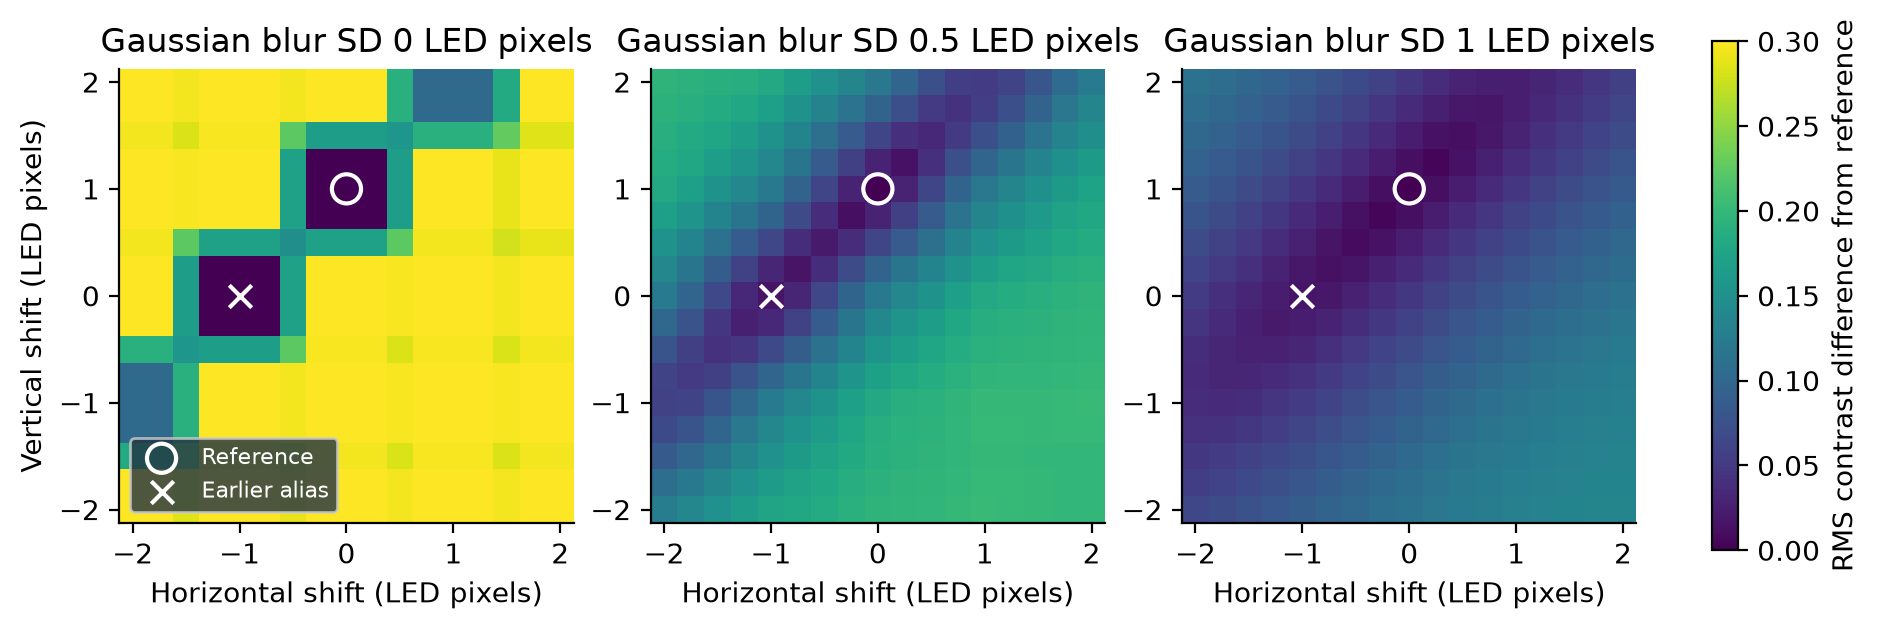
\includegraphics[width=\textwidth]{../../results/alignment_assessment_pilot_v1/figures/optical_sampling_sensitivity.png}
\caption{Input differences from the historical reference for cell 4 across 289 sampled shifts. Gaussian blur changes the pattern of input equivalence. The circle marks the reference and the cross an earlier integer alias. RMS contrast differences do not measure neural distinguishability.}
\end{figure}

\subsection{Retaining alignments reduces false rejection while often leaving assessment unresolved}

In the controlled spatial example, selecting a single calibration-optimal alignment frequently rejected the generating family (Table 2). At noise SD 0.02, this occurred in 8,989 of 15,000 generating-family assessments (59.93\%). The compatibility-set procedure rejected 692 (4.61\%), consistent with its conditional 5\% bound. However, only 370 assessments (2.47\%) were all-pass and 13,938 (92.92\%) remained unresolved. The oracle-alignment comparator rejected 363 (2.42\%).


Table 2. Generating-family assessment in the R2 synthetic benchmark. Every row includes 15,000 datasets balanced across three generating families and 25 true centres. Percentages describe this specified simulation design.


\begin{center}
\small
\begin{tabularx}{\textwidth}{l>{\centering\arraybackslash}X>{\centering\arraybackslash}X>{\centering\arraybackslash}X>{\centering\arraybackslash}X}
\toprule
\textbf{Noise SD} & \textbf{Single-fit rejection} & \textbf{Set rejection} & \textbf{Set unresolved} & \textbf{Oracle rejection} \\
\midrule
0.02 & 59.93\% & 4.61\% & 92.92\% & 2.42\% \\
0.05 & 36.71\% & 4.12\% & 68.99\% & 2.37\% \\
0.10 & 13.27\% & 4.05\% & 29.08\% & 2.47\% \\
\bottomrule
\end{tabularx}
\end{center}

Increasing noise reduced single-fit rejection, but this is not an improvement in recovery. Higher noise also reduces the ability of the independent test to detect differences between predictions. Similarly, a smaller unresolved rate at higher noise can arise because weak tests allow many alignments to pass. Neither trend should be interpreted as greater mechanistic certainty.


\subsection{Other model families are increasingly retained as noise rises}

Each dataset was also assessed under the two non-generating families. At noise SD 0.02, the set procedure did not reject 6,793 of 30,000 such assessments (22.64\%); 109 (0.36\%) were all-pass. At SD 0.10, 28,392 (94.64\%) were not rejected and 20,927 (69.76\%) were all-pass (Table 3). Retaining the generating model therefore does not establish useful discrimination among mechanisms. Figure 2 presents rejection and disposition rates together.


Table 3. Assessments of non-generating families. Each row includes 30,000 candidate-family assessments across 15,000 underlying datasets; these are not 30,000 independent experiments.


\begin{center}
\small
\begin{tabularx}{\textwidth}{l>{\centering\arraybackslash}X>{\centering\arraybackslash}X}
\toprule
\textbf{Noise SD} & \textbf{Other family not rejected by set} & \textbf{Other family all-pass} \\
\midrule
0.02 & 22.64\% & 0.36\% \\
0.05 & 84.11\% & 14.80\% \\
0.10 & 94.64\% & 69.76\% \\
\bottomrule
\end{tabularx}
\end{center}

\begin{figure}[htbp]
\centering
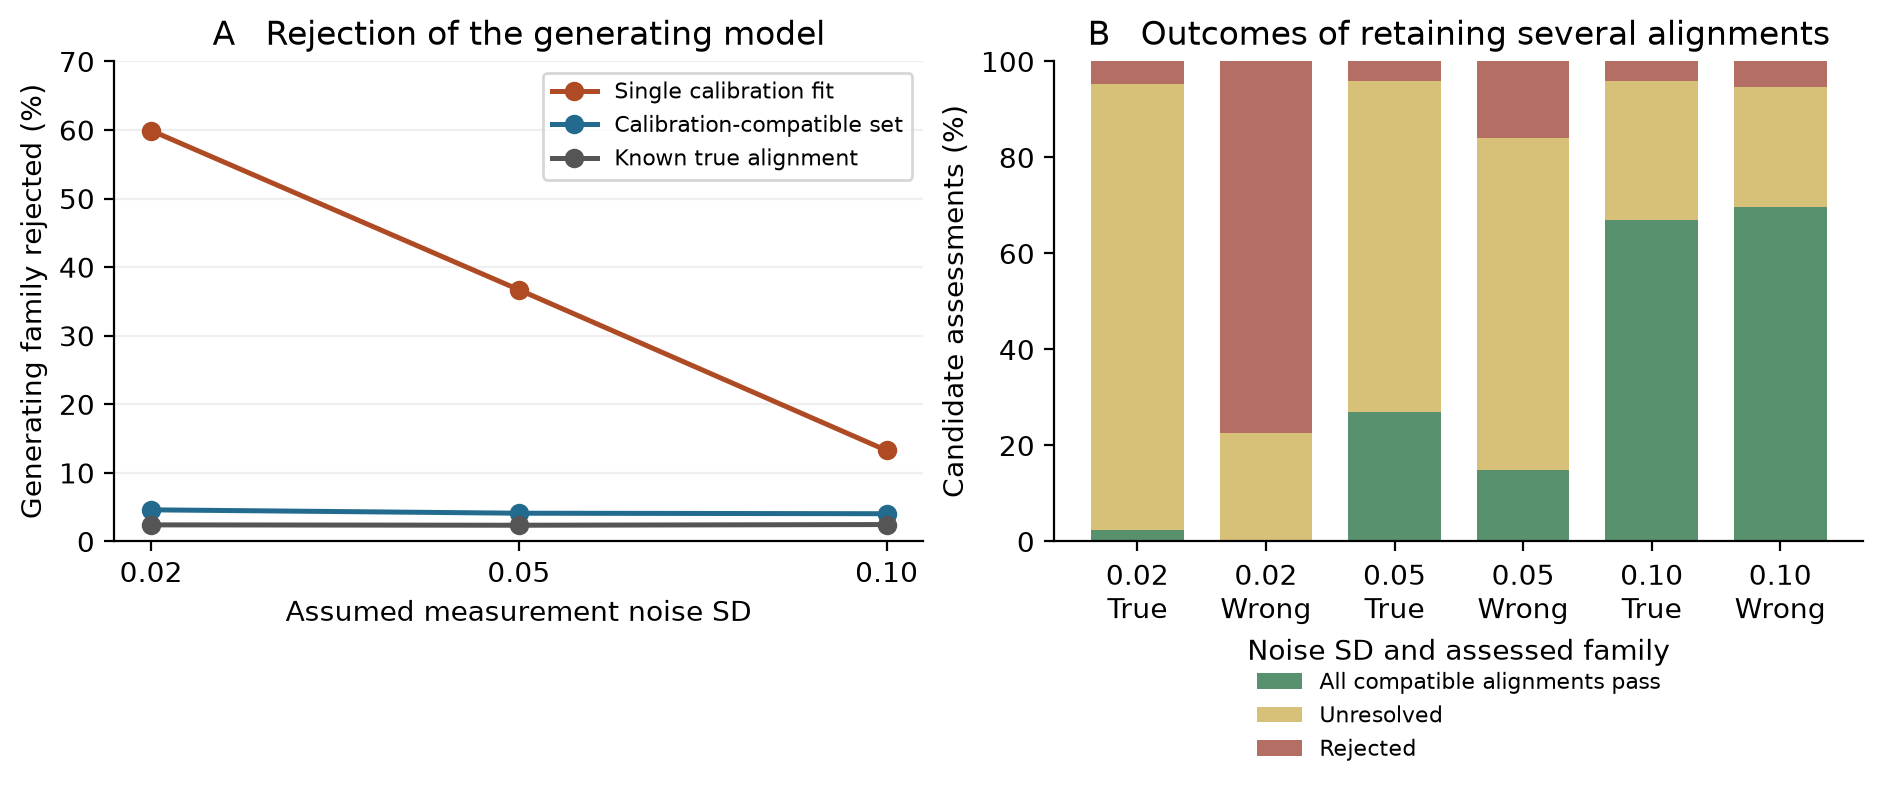
\includegraphics[width=\textwidth]{../../results/alignment_assessment_pilot_v1/figures/known_truth_assessment.png}
\caption{Controlled spatial-model assessment. A shows rejection rates for the generating family using one calibration fit, an alignment set, or the true alignment. B shows the set procedure's complete outcome distribution for generating and other families. All-pass denotes a finite known-noise test outcome, not recovery of a biological mechanism. Noise scales and filter families are synthetic.}
\end{figure}

\subsection{Numerical review supports the reported calculation and exposes tie sensitivity}

The amended independent review reproduced all 27 summary count rows across 135,000 candidate-family assessments. Maximum scalar contrast discrepancy over 810 checked image samples was $1.11\times10^{-16}$; selected independently recomputed statistics differed by at most $3.42\times10^{-13}$ chi-square units. Eight focused tests passed.


The tie amendment changed seven single-fit summary rows. For the pooled generating-family comparison at noise SD 0.02, rejection changed from 9,009 to 8,989 of 15,000; at SD 0.05, from 5,523 to 5,506; and at SD 0.10, from 1,991 to 1,990. Every compatibility-set and oracle count remained unchanged. The broad interpretation therefore did not depend on the amendment, although the initial exact single-fit counts were numerically unstable.


\section{Discussion}

This pilot places two limits on an initially attractive interpretation of a retrospective model mismatch. First, exact input equivalence in a piecewise-constant LED sampler need not survive a different optical observation model. Second, ambiguity in selected bar data cannot be extended to an experiment that also performed two-dimensional mapping without analyzing that additional information. The result is a correction to the scope of our reanalysis, not a demonstration that the published T4 experiment or model is invalid.


The synthetic example clarifies why reporting a range of plausible alignments can be useful and why that practice is insufficient for strong inference. Maintaining a set protects a generating model that would otherwise be tested at a poorly constrained calibration estimate. But it does not create the missing information: the response can remain unresolved, and alternative mechanisms can also survive. At high noise, even an all-pass outcome may be common for wrong families. A measure of usefulness must therefore consider discrimination and decisiveness together with error control.


These conclusions agree with established identifiability analysis [1,2], uncertainty-aware receptive-field modeling [4], and known-truth software validation [5]. They do not constitute new general identifiability theory. Our alignment set is a deliberately simple absolute-compatibility construction, not a substitute for established Bayesian or likelihood-based methods. We have not compared those methods, estimated noise from empirical trials, or demonstrated a novel decision rule with superior performance.


The distinction between input uncertainty and dynamical uncertainty is also important. Studies of connectome-constrained networks investigate what structural information and recordings can determine about neural activity [7,9]. Our raw-image analysis addresses a different component: delivery of spatial inputs to a fixed modeled cell. It cannot establish neural degeneracy, explain the dynamics of the complete motion circuit, or identify how flies detect small turns during walking. The six archived cells also come from one previously examined source dataset, so they do not establish broad prevalence across experiments or laboratories.


Adding an explicit blur is not automatically an appropriate correction to a model whose effective spatial inputs were fitted to receptive-field responses. It can overlap with spatial filtering already absorbed into those parameters. We did not refit the cable or determine whether such double counting would occur here. The optical analysis establishes sensitivity to a specified input assumption, not a physiologically preferred preprocessing pipeline.


A stronger next study would first obtain independent constraints on the optical and response observation models and incorporate the complete original mapping information where available. A proposed calibration remedy would then need comparison with conventional two-dimensional mapping and established uncertainty-aware assessment, under the same presentation budget and with predeclared recovery outcomes. Optimizing stimuli to distinguish mechanisms has extensive prior work [10-12]. The present results do not demonstrate that another custom calibration procedure would improve upon it.


\section{Conclusion}

The original exact-alignment observation is reproducible under its stated LED sampler but does not survive the wider assumed Gaussian blur on the sampled grid. A separate known-truth example shows that propagating alignment uncertainty can reduce rejection of a correct family while leaving many assessments unresolved or retaining incorrect families. This pilot supports explicit sensitivity analysis and restrained interpretation. It does not yet establish a new calibration method, a general biological ambiguity, or a validated explanation of fly motion processing.


\section{Data and code availability}

The source T4 data are available at \url{https://doi.org/10.25378/janelia.5576101}. This draft's scripts, frozen protocols, source-hash records, image banks, simulation summaries, numerical amendment and reviews are retained in the accompanying project archive \texttt{results/\allowbreak{}alignment\_\allowbreak{}assessment\_\allowbreak{}pilot\_\allowbreak{}v1}. The original and corrected simulation outputs are both preserved. No public release or new archival DOI for the present reanalysis is claimed.


The image audit consumed 4.70 process CPU seconds and peaked at 579,928,064 bytes RSS; the initial synthetic stage consumed 1.37 CPU seconds and peaked at 112,427,008 bytes RSS. These independent single-process stages ran concurrently, contrary to the protocol's one-process wording; combined instantaneous RSS was not measured. Subsequent correction and review used separate processes. No new recordings, NEURON simulations or movie archive were generated. Work resumed after laptop suspension by checking the saved source locks before manuscript preparation.


\section{Author declarations}

This analysis used existing public recordings and synthetic data; no new animal experiment was performed. Authorship and contributions, institutional affiliations, funding, conflicts of interest, required ethics statements and any required disclosure of computational assistance remain for investigator review. This draft has not been submitted or accepted for publication.


\section{References}

\noindent\hangindent=1.5em\hangafter=1 1. Thomas J. Rothenberg (1971). Identification in Parametric Models. \emph{Econometrica} 39, 577-591. \href{https://doi.org/10.2307/1913267}{doi:10.2307/1913267}\par\smallskip

\noindent\hangindent=1.5em\hangafter=1 2. A. Raue, C. Kreutz, T. Maiwald, J. Bachmann, M. Schilling, U. Klingmuller, J. Timmer (2009). Structural and practical identifiability analysis of partially observed dynamical models by exploiting the profile likelihood. \emph{Bioinformatics} 25, 1923-1929. \href{https://doi.org/10.1093/bioinformatics/btp358}{doi:10.1093/bioinformatics/btp358}\par\smallskip

\noindent\hangindent=1.5em\hangafter=1 3. Serge O. Dumoulin, Brian A. Wandell (2008). Population receptive field estimates in human visual cortex. \emph{NeuroImage} 39, 647-660. \href{https://doi.org/10.1016/j.neuroimage.2007.09.034}{doi:10.1016/j.neuroimage.2007.09.034}\par\smallskip

\noindent\hangindent=1.5em\hangafter=1 4. Peter Zeidman, Edward Harry Silson, Dietrich Samuel Schwarzkopf, Chris Ian Baker, Will Penny (2018). Bayesian population receptive field modelling. \emph{NeuroImage} 180, 173-187. \href{https://doi.org/10.1016/j.neuroimage.2017.09.008}{doi:10.1016/j.neuroimage.2017.09.008}\par\smallskip

\noindent\hangindent=1.5em\hangafter=1 5. Garikoitz Lerma-Usabiaga, Noah Benson, Jonathan Winawer, Brian A. Wandell (2020). A validation framework for neuroimaging software: The case of population receptive fields. \emph{PLoS Computational Biology} 16, e1007924. \href{https://doi.org/10.1371/journal.pcbi.1007924}{doi:10.1371/journal.pcbi.1007924}\par\smallskip

\noindent\hangindent=1.5em\hangafter=1 6. Eyal Gruntman, Sandro Romani, Michael B. Reiser (2018). Simple integration of fast excitation and offset, delayed inhibition computes directional selectivity in Drosophila. \emph{Nature Neuroscience} 21, 250-257. \href{https://doi.org/10.1038/s41593-017-0046-4}{doi:10.1038/s41593-017-0046-4}\par\smallskip

\noindent\hangindent=1.5em\hangafter=1 7. J. K. Lappalainen, F. D. Tschopp, S. Prakhya, et al. (2024). Connectome-constrained networks predict neural activity across the fly visual system. \emph{Nature} 634, 1132-1140. \href{https://doi.org/10.1038/s41586-024-07939-3}{doi:10.1038/s41586-024-07939-3}\par\smallskip

\noindent\hangindent=1.5em\hangafter=1 8. Arthur Zhao, Eyal Gruntman, Aljoscha Nern, et al. (2025). Eye structure shapes neuron function in Drosophila motion vision. \emph{Nature} 646, 135-142. \href{https://doi.org/10.1038/s41586-025-09276-5}{doi:10.1038/s41586-025-09276-5}\par\smallskip

\noindent\hangindent=1.5em\hangafter=1 9. Manuel Beiran, Ashok Litwin-Kumar (2025). Prediction of neural activity in connectome-constrained recurrent networks. \emph{Nature Neuroscience} 28, 2561-2574. \href{https://doi.org/10.1038/s41593-025-02080-4}{doi:10.1038/s41593-025-02080-4}\par\smallskip

\noindent\hangindent=1.5em\hangafter=1 10. Liam Paninski (2005). Asymptotic theory of information-theoretic experimental design. \emph{Neural Computation} 17, 1480-1507. \href{https://doi.org/10.1162/0899766053723032}{doi:10.1162/0899766053723032}\par\smallskip

\noindent\hangindent=1.5em\hangafter=1 11. Jeremy Lewi, Robert Butera, Liam Paninski (2009). Sequential optimal design of neurophysiology experiments. \emph{Neural Computation} 21, 619-687. \href{https://doi.org/10.1162/neco.2008.08-07-594}{doi:10.1162/neco.2008.08-07-594}\par\smallskip

\noindent\hangindent=1.5em\hangafter=1 12. Tal Golan, Heiko H. Schütt, Nikolaus Kriegeskorte (2026). Making models disagree to learn how brains compute. \emph{Nature Reviews Neuroscience} 27, 767-788. \href{https://doi.org/10.1038/s41583-026-01070-0}{doi:10.1038/s41583-026-01070-0}\par\smallskip
\end{document}
